\documentclass[../main.tex]{subfiles}

\chapter{Hardware}
\section{Atomic Clock}\label{hw_csac}
\begin{wrapfigure}{c}{0.45\textwidth}
  \centering
  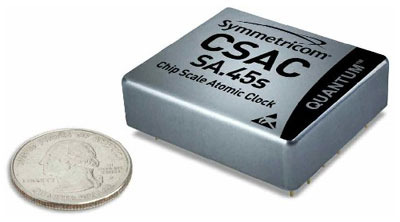
\includegraphics[width=0.40\textwidth]{csac.jpg}
  \caption[Symmetricom SA.45s CSAC]
   {Symmetricom SA.45s CSAC. Courtesy Symmetricom.}
\end{wrapfigure}
We decided to use the Symmetricom SA.45 as the atomic clock. This is an atomic clock measuring only 16cc with 1 pulse per second (PPS) output and 1 PPS input for disciplining. The SA.45's strength is its low power consumption (less than 120mW) and low price. The SA.45 also uses a built-in controller which can be communicated with over a RS-232 serial interface. The ability to communicate with the atomic clock, issue commands and collect data is paramount for the feasibility of our proposal. It is worth mentioning that any atomic clock, such as Cesium standard or even a Rubidium standard, could be used given that they have a means to communicate basic telemetry like phase difference and steer values and can configured by wire to change modes of disciplining. For more about clock performance, review the SA.45s' user guide \cite{CSAC_USERGUIDE} and data sheet \cite{SADS}.

\section{Atomic clock controller platform}\label{platform}
We chose to cast the Raspberry Pi 3 Model B (RASPI3) in the role as the host running the atomic clock controller software. The RASPI3 is an interesting piece of equipment with an impressive list of specifications. It is a single board computer with a 1.2GHz 64-bit quad-core ARMv8 CPU, 1 GB of RAM, built-in 802.11n Wireless LAN and four USB ports \cite{RASPI}. As with the Symmetricom SA.45, the RASPI3 is very affordable. The RASPI3 retailed at about 35 USD when this report was written. We also propose to use Raspbian \cite{RASPBIAN}, a Debian derived flavor of Linux optimized for the Raspberry Pi, as the operating system. 

\section{GPS receiver}
We chose to use at least two GPS receivers. Both of the receivers should collect data and feed it to the atomic clock controller, but one of the receivers should also double as a 1 PPS disciplining source for the atomic clock. Considering the need for a stable 1 PPS source, we propose to use the u-blox NEO-M8T. This is a relativity affordable GPS receiver with a temperature compensated crystal oscillator (TCXO), 3 concurrent GPS reception and an external antenna \cite{UBLOXM8T}. In the current implementation of the atomic clock controller, only NMEA data is collected from the GPS receivers (see section \ref{nmea_data} for more about NMEA data). However in the future it might be beneficial to collect and process raw data\footnote{The ublox M8T is capable of outputting RAW data. This is for example used by RTKLIB (http://www.rtklib.com/) instead of NMEA} from the receivers as well. Since most GPS receivers today follow the NMEA standard (to some extent) and raw data currently is not required, common and popular receivers like the u-blox NEO series should be more than sufficient for use in our implementation.

\subsection{GPS receiver configuration}
According to the u-blox NEO-M8T's manual \cite{UBLOXM8TMANUAL}, the device includes a feature called \textit{Fixed Position}. This is a feature that must be enabled in order to put the device in \textit{Time Mode}. This feature makes the device solve time with higher certainty even with fewer available satellites. The \textit{Time mode} was not used, relied on or accounted for, in our solution. 